\documentclass{article}
\usepackage{amsmath}
\usepackage{amssymb}
\usepackage{graphicx}
\usepackage{hyperref}
\usepackage[version=4]{mhchem}


\begin{document}
(1997 China Middle School Math Contest) In trapezoid \(A B C D, \angle B\) \(=30^{\circ}, \angle C=60^{\circ}\). Find \(E F\) if \(B C=7, M N=3\). \(E, M, F, N\) are the midpoint of \(A B, B C, C D, D A\), respectively.\\
(A) 4\\
(B) \(4 \frac{1}{2}\) (C) 5\\
(D) 6\\
\centering
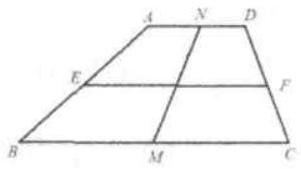
\includegraphics[width=\textwidth]{images/116(2).jpg}

Solution: (A).\\
Draw \(N G / / A B\) to meet \(B C\) at \(G, N H / / D C\) to meet \(B C\) at H.

So both \(A B G N\) and \(D C H N\) are parallelograms.\\
Since \(\angle B+\angle C=90^{\circ}, \angle N G H+\angle N H G=90^{\circ}\).\\
\centering
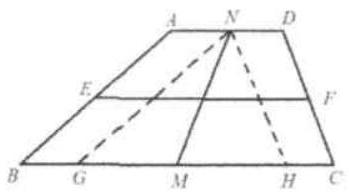
\includegraphics[width=\textwidth]{images/116(1).jpg}

Since \(B G=A N=N D=H C, B M=M C\). So \(G M=M H\).\\
In right triangle \(G N H, G H=2 M N=6\).


So \(A D=B C-G H=1\).\\
Thus \(E F=\frac{1}{2}(A D+B C)=4\).\\
The answer is (A).


\end{document}
